\section{Spørsmål Runde 2 }
Programmet som jeg bruker til å lese av grafene \textbf{Engauge Digitizer}.  
Lagde en kjapp oversikt før jeg startet. Bare legger den med, hvis du ikke er interessert er det bare å ignorere 
denne seksjonen:
\subsection{Engauge Digitizer, General Steps}
\textbf{Typical Steps:}
\begin{enumerate}
   \item Obtain image file (bmp, jpeg or other) showing one or more curves and both axes;
   \item Import image file using either:
      \begin{itemize}
         \item File/Import menu option;
         \item Copy-Paste;
         \item Drag and drop;
      \end{itemize}
   \item If important parts of the image is missing (e.g. parts of- or entire curves) or 
      curves are too thick (difficult to separate them),
      then go to \texttt{Settings/Discretize} and experiment with the discretization options
      until all curves are there and looking as nice as possible.
   \item Click on \texttt{Axes Point} button. 
   \item Click on click on one of the axes and enter graph coordinates.\\
         Repeat until you've added all axes (''origin'', point on x-axis and point on y-axis);
   \item Digitize graph: Click on the \texttt{Segment Fill} button to automatically digitize entire curve
         segments at a time or Click on the \texttt{Point Match} button to automatically digitize many 
         curve points. Click on a sample point and use the arrow keys to accept or reject points that match
      the sample point.


   \item Click on the \texttt{Curve Points} button to manually enter curve points by 
      clicking on the curve. Repeat until the curve is covered with a sufficient number of curve points.
   \item Export curve points by using either: 
      \begin{itemize}
         \item File/Export menu option to save selected curves into a tabular text file, or
         \item copy-pase / drag-drop points in the current curve from mthe \texttt{curve geometry window}
               to another application.
         \item Copy-Paste;
         \item Drag and drop;
      \end{itemize}
\end{enumerate}
Hær er et lite bilde av hvordan det importerte bildet set ut i engauge:
\begin{wrapfigure}{r}{0.6\textwidth} %Requires the package wrapfigure
  \begin{center}
    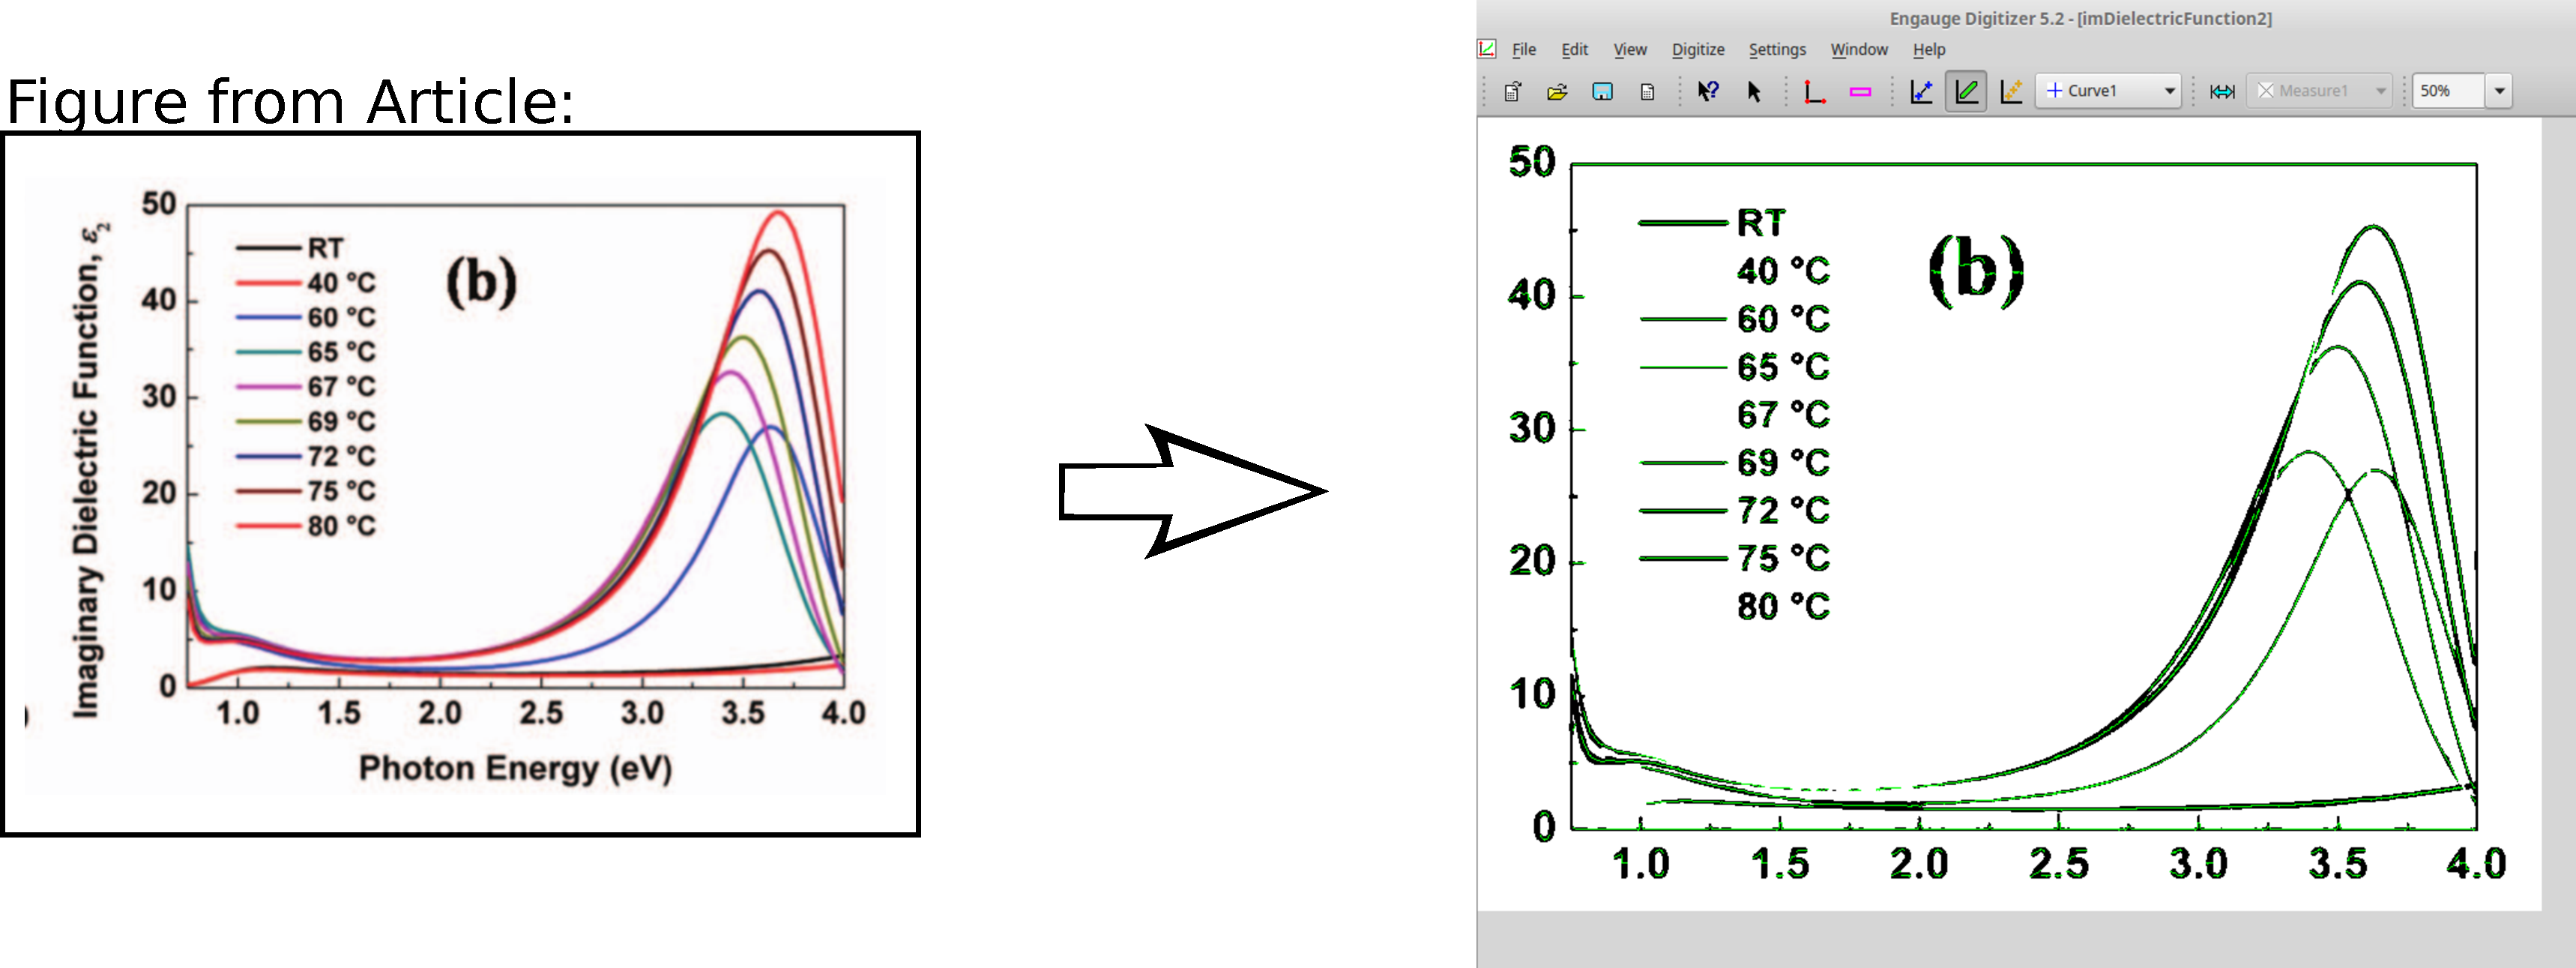
\includegraphics[width=0.58\textwidth]{engaugeExample.pdf}
  \end{center}
\end{wrapfigure}
%

\newpage
\subsection{Får ikke til å bruke scipy.interpolate funksjonene}
Jeg har prøvd å ekvidistansere datapunktene mine og intrapolere ved å bruke 
scipy.interp1d og scipy.griddata. Problemet er at jeg vil bare intrapolere
verdiene for det intervallet av x-verdiene der dataen for n- og k-verdiene overlapper.
Dette gjør at jeg ikke kan bruke de ovenfornevnte funksjonene, siden dimensjonene på
arrayene ikke stemmer. Hær er koden jeg har prøvd å bruke:
\newline
\begin{lstlisting}[style=FormattedNumber,frame=none, language=python]
#!/usr/bin/python
import numpy
#from scipy.interpolate import interp1d 
from scipy.interpolate import griddata

def find_nearest(array,value):
    i = (numpy.abs(array-value)).argmin()
    return i

#Of the largest min-values in the two arrays, this functions finds the index in the other array
# corresponding to this value:
def find_min_x(x1, x2): 
    if( x1[0] < x2[0] ):
        imin = find_nearest(x1, x2[0])
        if( x1[imin] < x2[0] ):
            imin = imin + 1
            return x1[imin]
        else: 
            return x2[0]
    else:
        imin = find_nearest(x2, x1[0])
        if( x2[imin] < x1[0]):
            imin = imin + 1
            return x2[imin]
        else:
            return x1[0]


def find_max_x(x1, x2): 
    if( x1[-1] < x2[-1] ):
        imax = find_nearest(x2, x1[-1])
        if( x1[-1] < x2[imax] ):
            imax = imax - 1
            return x2[imax]
        else: 
            return x1[-1]
    else:
        imax = find_nearest(x1, x2[-1])
        if( x2[-1] < x1[imax] ):
            imax = imax - 1
            return x1[imax]
        else: 
            return x2[-1]

\end{lstlisting}
%
\newpage
\begin{figure}[h!] 
\centering 
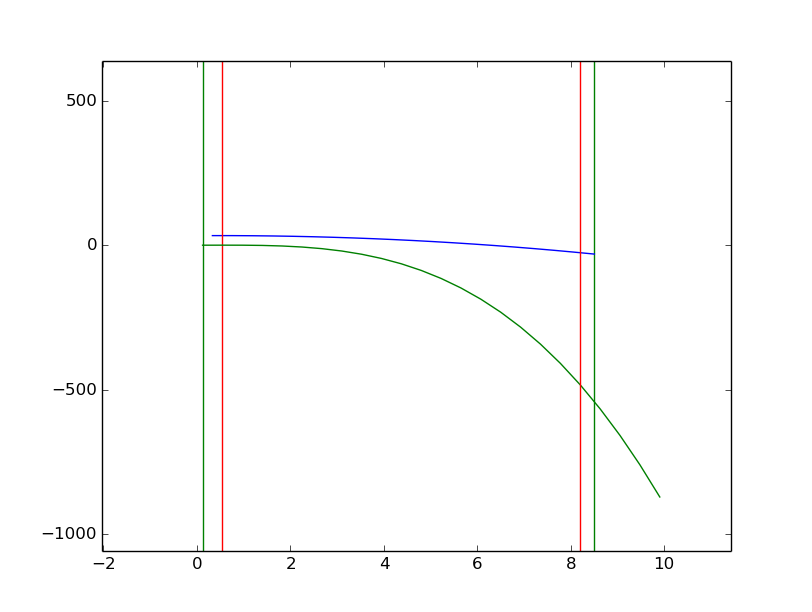
\includegraphics[width=0.5\textwidth]{dataBoundaries.png} 
\caption{Jeg bruker find\_nearest(), find\_min\_x() and find\_max\_x() for å finne hvor datapunktene 
overlapper og tar den første og siste verdien innenfor dette området. Disse verdiene brukes som
start og slutt verdi for energi/bølgelengde og vil bli skrevet ut i første linje av ''.nk'' filen. 
Denne grafen er bare en test for å se at funksjonene virker.} 
\end{figure}

Koden fortsetter:
\begin{lstlisting}[style=formattednumber,frame=none, language=python]
skipRows = 1 #input for numpy.loadtxt(). Skips the first row with the top information
valueDelimiter = ',' # input for numpy.loadtxt(). Tells which symbol that separates the data


unit = 2 #OUTPUT-LINE-1, x = wavelength
nData = numpy.loadtxt('reOpticalIndexVO2.csv', skiprows=skipRows, delimiter=valueDelimiter)
kData = numpy.loadtxt('imOpticalIndexVO2.csv', skiprows=skipRows, delimiter=valueDelimiter)

# Find lowest x-value which are in both datasets:
x1 = find_min_x(nData[0], kData[0])

# Find largest -value which are in both datasets:
x2 = find_max_x(nData[0], kData[0])

#Not sure about the number of data points so I just use the lowest of the two:
dataPoints = 150 #OUTPUT-LINE-1

firstLine = str(unit)+'\t'+str(x1)+'\t'+str(x2)+'\t'+str(dataPoints)  

# Interpolate the data such that we get the n,k values for the same equidistant x-values:
x = numpy.linspace(x1,x2, num=dataPoints, endpoint=True) #equidistant x-values
#try 1:
#n = interp1d(x,nData[:,1])
#k = interp1d(x,kData[:,1])
#try 2:
#n = griddata(nData[:,0], nData[:,1], x, method='linear')
#k = griddata(kData[:,0], kData[:,1], x, method='linear')

#write to file
numpy.savetxt('savetxtOutput.nk', numpy.column_stack((n,k)), delimiter='\t', header=firstLine, comments='')
#comments='' because if not, then the header would be a comment and contain the #-symbol
\end{lstlisting}

Feilmeldingene jeg får for å bruke interp1d() er: 
\begin{lstlisting}[style=formattednumber,frame=none, language=bash]
Traceback (most recent call last):
  File "./convertData.py", line 105, in <module>
      n = interp1d(x,nData[:,1])
  File "/usr/lib/python2.7/dist-packages/scipy/interpolate/interpolate.py", line 333, in __init__
      _Interpolator1D.__init__(self, x, y, axis=axis)
  File "/usr/lib/python2.7/dist-packages/scipy/interpolate/polyint.py", line 35, in __init__
      self._set_yi(yi, xi=xi, axis=axis)
  File "/usr/lib/python2.7/dist-packages/scipy/interpolate/polyint.py", line 94, in _set_yi
      raise ValueError("x and y arrays must be equal in length along "
ValueError: x and y arrays must be equal in length along interpolation axis.
\end{lstlisting}

Bruker jeg griddata() får jeg ingen feilmeldinger, men outputfilen min ser slik ut:
\begin{lstlisting}[style=formattednumber,frame=none, language=bash]
2	0.0607533	2.23613	150
nan	nan
nan	nan
nan	nan
nan	nan
nan	nan
nan	nan
nan	nan
nan	nan
nan	nan
nan	nan
\end{lstlisting}
Det er åpenbart at jeg prøver å gjøre noe som ikke er lov i første tilfellet og i andre tilfellet 
har jeg kanskje misforstått helt. Tenkte bare å høre om det jeg har startet å gjøre 
er fornuftig og om du hadde noen tips til hvordan jeg kan gå frem videre? Hvordan jeg evt.
kan løse problemet eller gå rundt det.
